\documentclass{beamer}
\usetheme{Boadilla}
\title[Semester Project]{Rigorous data-driven computation of spectral properties of Koopman operators for dynamical systems}
\author[Ivan Bioli]{\emph{Author}: Ivan Bioli\\[5mm]{\emph{Professor}: Daniel Kressner \\ \emph{Supervisor}: Alice Cortinovis}}
\institute[EPFL]{École Polytechnique Fédérale de Lausanne\\Master in Computational Sciences and Engineering}
\date{May 30, 2022}
\usepackage{preamble_presentation}
\setbeamertemplate{caption}{\insertcaption}

\begin{document}
\begin{frame}
\centering
\titlepage
\end{frame}

\begin{frame}[fragile]{The Koopman Operator}
Autonomous dynamical systems with finite-dimensional state space and discrete time steps:
\begin{equation*}
    \vb{x}_{n+1} = \vb{F}(\vb{x}_n)\,\,\,n\geq 0, \qquad \vb{F}:\Omega \to \Omega
\end{equation*}
\begin{definition}[Observable]
A function $g:\Omega\to\C$ used to indirectly measure the state of the dynamical system is called an observable. 
\end{definition}
\begin{definition}[Koopman Operator]
Given a suitable domain of observables $\mathcal{D}(\mathcal{K}) \subseteq L^2(\Omega)$ we define the Koopman Operator as:
\begin{equation*}
    \label{koopman_def}
    \begin{split}
       \mathcal{K} : \mathcal{D}(\mathcal{K}) &\longrightarrow L^2(\Omega, \omega)
       \\
       g & \longmapsto g \circ \vb{F}
    \end{split}    
\end{equation*} 
\end{definition}
\end{frame}

\begin{frame}[fragile]{Linear dynamical systems}
\centering
$\vb{F}(\vb{x}) = A\vb{x}$, $\vb{A}\in\R^{d\times d}$
\begin{prop}
Let us assume that $\vb{A}\in\R^{d\times d}$ is diagonalizable with a full set of eigenpairs $\{(\lambda_j, \vb{v}_j)\}_{j=1}^{d}$. Let $\{(\overline{\lambda}_j, \vb{w}_j)\}_{j=1}^{d}$ be the eigenpairs of of $\vb{A}^*$, with $\{\vb{w}_j)\}_{j=1}^{d}$ such that $\langle \vb{v}_j, \vb{w}_k\rangle = \delta_{k,j}$. Then we can rewrite $\vb{x}\in\R^d$:
\begin{equation*}
    \label{decomposition_linear}
    \vb{x} = \sum_{j=1}^d \langle \vb{x}, \vb{w}_j\rangle \vb{v}_j = \sum_{j=1}^d \phi_j(\vb{x}) \vb{v}_j.
\end{equation*}
It holds $[\mathcal{K}\phi_j](\vb{x}) = \lambda_j\phi_j$ and the evolution of the system reads
\begin{equation*}
    \label{evolution_linear}
    \vb{F}(\vb{x}) = \vb{A}\vb{x}  = \sum_{j=1}^d \phi_j(\vb{x}) \vb{A}\vb{v}_j = \sum_{j=1}^d \lambda_j \phi_j(\vb{x}) \vb{v}_j = \sum_{j=1}^d [\mathcal{K}\phi_j](\vb{x})\vb{v}_j.
\end{equation*}
\end{prop}
\end{frame}

\begin{frame}[fragile]{Nonlinear dynamical systems}
\begin{definition}[Koopman Mode Decomposition]
$g:\Omega\to\C^p$ a vector valued observable s.t. each of its component $g_i$ lies in the closure of the Span of $J$ Koopman eigenfunctions, where the case $J=+\infty$ is possible (and often occurs). Then we can write $\displaystyle{g_i = \sum_{j = 1}^J v_{ij}\phi_j, \, v_{ij}\in\C}$ and staking the weights into the vectors 
%$\vb{v}_j = [v_{1j},\dots,v_{pj}]^T\in\C^p$ 
\begin{equation*}
    \label{koopman_modes}
	g(\vb{x}) = \sum_{j = 1}^J \phi_j(\vb{x})\vb{v}_{j}.
\end{equation*}
\end{definition}
\begin{itemize}
    \item $\vb{F}(\vb{x}) = [\mathcal{K}g](\vb{x}) = \sum_{j = 1}^J [\mathcal{K}\phi_j](\vb{x})\vb{v}_j = \sum_{j = 1}^J \lambda_j\phi_j(\vb{x})\vb{v}_j$
    \item $g(\vb{x}_n) = [\mathcal{K}^ng](\vb{x}_0) = \sum_{j = 1}^J \lambda_j^n\phi_j(\vb{x}_0)\vb{v}_{j}$ 
    \item Idea: link the two formulations via the full state observable $g(x) = x$
\end{itemize}
\end{frame}

\begin{frame}[fragile]{Dynamic Mode Decomposition (DMD)}
Linear dynamical system: $x_{n+1} = Ax_n$. Access to a sequence of snapshots:
\begin{equation*}
    \vb{V}_1^N = \left[\vb{v}_1, \vb{v}_2, \dots, \vb{v}_N\right] = \left[\vb{v}_1, \vb{A}\vb{v}_1, \dots, \vb{A}^N\vb{v}_1\right]
\end{equation*}
\alert{\textbf{Idea:}} write $\vb{v}_N = a_1 \vb{v}_1 + \dots + a_{N-1} \vb{v}_{N-1} + \vb{r}$ and minimize the residual.
\begin{block}{DMD (Arnoldi-based version)}
\begin{equation*}
    \vb{A}\vb{V}_1^{N-1}  = \vb{V}_1^{N-1}\vb{S} + \vb{r}\vb{e}_{N-1}^T, \quad 
    \vb{S} :=
   \begin{bmatrix}
   0     &        &       &      & a_1 \\
   1     & 0      &       &      & a_2 \\
         & \ddots & \ddots&      & \vdots \\ 
         &        & 1     & 0    & a_{N-2} \\
         &        &       & 1    & a_{N-1} \\
   \end{bmatrix}.
\end{equation*}
To minimize the norm of the residual $\vb{V}_1^{N-1} = \vb{Q}\vb{R}$ and:
\begin{equation*}
    \vb{a} = \vb{R}^{-1} \vb{Q}^*\vb{v}_N = (\vb{V}_1^{N-1})^{\dagger}\vb{v}_N.
\end{equation*}
\end{block}
\end{frame}

\begin{frame}{DMD and the Arnoldi method}
\begin{prop}
Suppose that $\vb{V}_1^{N-1}$ is of full column rank. Then the Arnoldi method and the DMD algorithms are equivalent in exact arithmetic, i.e. the Ritz pairs returned by the two algorithms coincide. 
\end{prop}
\alert{\textbf{But:}} the Arnoldi method is more stable as does not compute the iterates explicitly. A SVD-based version of the DMD algorithm improves numerical stability (and is equivalent in exact arithmetic).
\begin{figure}[h]
    \begin{columns}
        \column{.45\linewidth}
        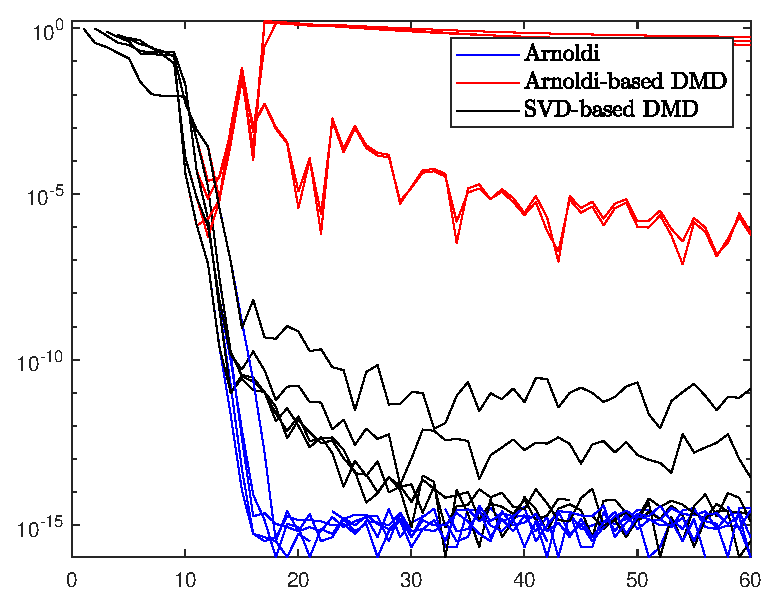
\includegraphics[width=\linewidth]{../code/figures/Arnoldi_vs_DMD.eps}
        \column{.5\linewidth}
        \caption{Convergence of the five dominant eigenvalues using a matrix \texttt{A} of size \texttt{n = 400} defined as:\\ \texttt{A = diag([1, 0.9, 0.8.\^{}(1:n-2)])}.}
      \end{columns}
\end{figure}
\end{frame}

\begin{frame}{Extended Dynamic Mode Decomposition (EDMD)}
\alert{\textbf{Idea:}} approximate the Koopman Operator as a finite dimensional operator and then approximate the Koopman (eigenvalue, eigenfunction, mode) tuples from this finite dimensional approximation. 

\medskip
\structure{\textbf{Input}}:
\begin{itemize}
    \item Snapshot pairs of the system state: $\{(\vb{x}_0^{(m)}, \vb{x}_1^{(m)})\}_{m = 1}^M$ with $\vb{x}_1^{(m)} = \vb{F}(\vb{x}_0^{(m)})$;
    \item a dictionary of observables $\mathcal{D} = \{\psi_1, \dots, \psi_K\} \subseteq \mathcal{D}(\mathcal{K})$.
\end{itemize}
\end{frame}

\begin{frame}{A 1D example: the Gauss iterated map}
\begin{equation*}
    F:\Omega = [-1, 0] \to\Omega, \qquad F(x) =\exp(\alpha x^2) + \beta 
\end{equation*}
We consider:
\begin{itemize}
    \item $\{\vb{x}_0^{(m)}\}_{m = 1}^M$: Gauss-Legendre quadrature nodes, $M = 100$.
    \item Dictionary of observable $\mathcal{D}$: first $K = 40$ normalized Legendre polynomials, transplanted to $\Omega$.
\end{itemize}
\begin{figure}[h]
    \centering
    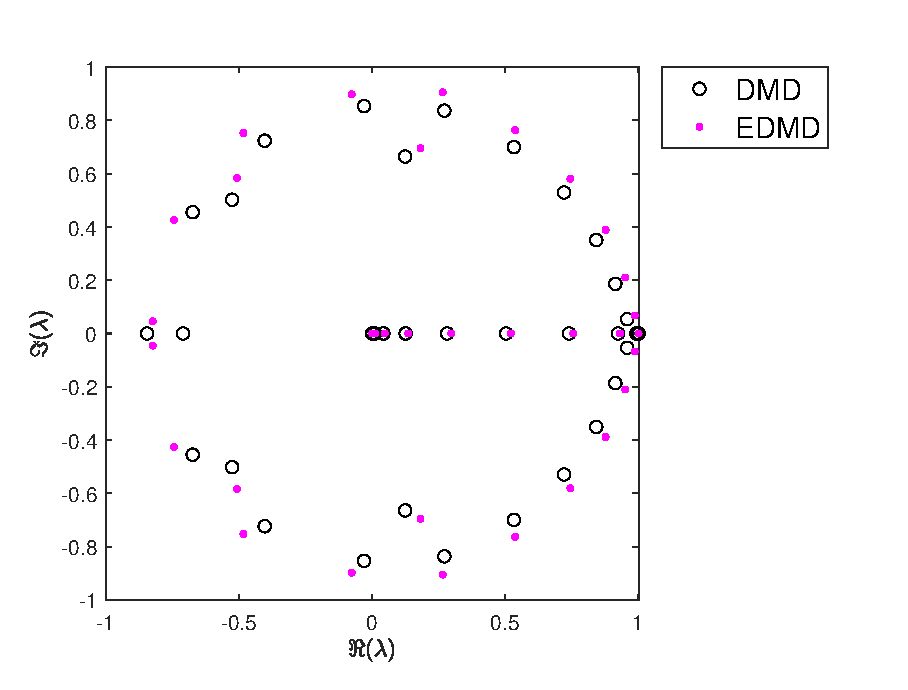
\includegraphics[width=0.55\linewidth]{../code/figures/gauss_map/presentation.eps}
\end{figure}
\end{frame}

\begin{frame}{Spectral pollution and Residual DMD (ResDMD)}
\alert{\textbf{Problem:}} Spurious eigenvalues only due to the discretization of $\mathcal{K}$.

\medskip
\only<1->{
\structure{\textbf{ResDMD}}: For each candidate eigenpair $(\lambda, \phi)$ of $\mathcal{K}$, approximate using the datapoints as quadrature nodes the residual:
\begin{equation*}
    \mathrm{res}(\lambda, \phi)^2 = \frac{\int_{\Omega} \abs{[\mathcal{K}\phi](x) - \lambda\phi(x)}^2\,\,d\omega(x)}{\int_{\Omega} \abs{\phi(x)}^2\,\,d\omega(x)} 
        = \frac{\langle (\mathcal{K} - \lambda \cdot\mathrm{id})\phi, (\mathcal{K} - \lambda \cdot \mathrm{id})\phi \rangle}{\langle\phi , \phi \rangle}
\end{equation*}
and discard if the residual is above a given tolerance $\varepsilon$.}
\begin{figure}[h]
    \centering
    \only<1>{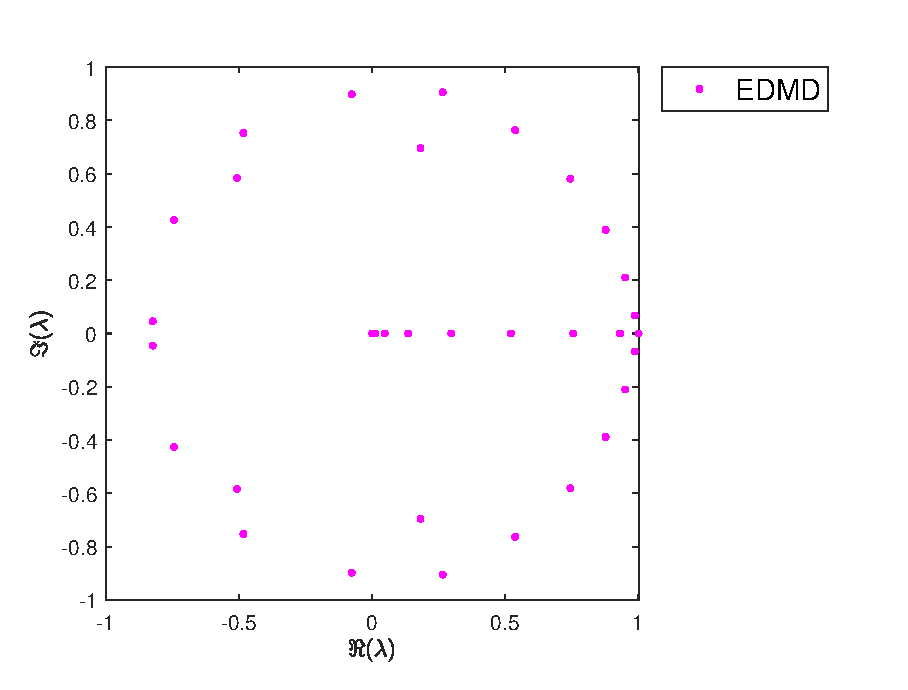
\includegraphics[width=0.53\linewidth]{../code/figures/gauss_map/presentation_edmd.eps}}
    \only<2>{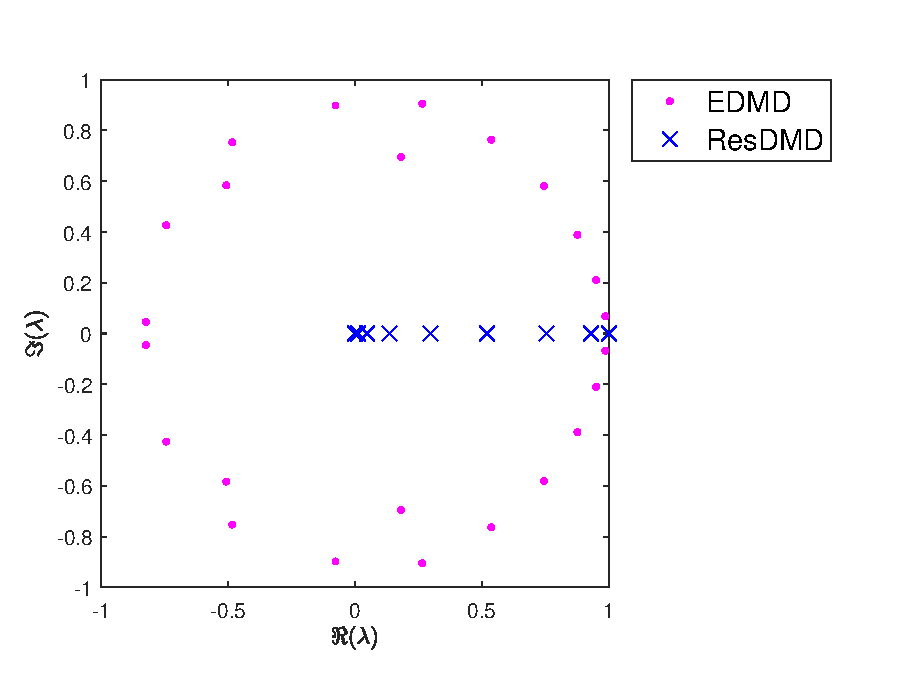
\includegraphics[width=0.53\linewidth]{../code/figures/gauss_map/presentation_resdmd.eps}}
\end{figure}
\end{frame}

\begin{frame}{ResDMD to approximate the pseudospectrum}
\only<1>{
\begin{definition}[Pseudospectrum]
\begin{itemize}
    \item Square matrices: $\displaystyle{\sigma_{\varepsilon}(\vb{A}) = \left\{ \lambda\in\C \text{ : } \norm{(\vb{A} - \lambda \vb{I})^{-1}}_2 \geq \frac{1}{\varepsilon}\right\}}$
    %\item Rectangular pencils: $\displaystyle{\sigma_{\varepsilon}(\vb{A}, \vb{B}) = \left\{ \lambda\in\C \text{ : } \sigma_{\mathrm{min}}(\vb{A} - \lambda \vb{B}) \leq \varepsilon \right\}}$
    \item Koopman Operator: $\displaystyle{\sigma_{\varepsilon}(\mathcal{K}) = \mathrm{cl}\left( \left\{ \lambda\in\C \text{ : } \norm{(\mathcal{K} - \lambda \cdot \mathrm{id})^{-1}} \geq \frac{1}{\varepsilon}\right\} \right)}$
\end{itemize}
\end{definition}

\structure{\textbf{ResDMD for pseudospectrum approximation:}} For each $\lambda$ on a grid, compute the function $\phi\in\Span(\mathcal{D})$ that minimizes (an approximation of) $\mathrm{res}(\lambda, \phi)$ and keep $\lambda$ if $\mathrm{res}(\lambda, \phi)<\varepsilon$.
\begin{prop}[\cite{colbrook_rigorous_2021}, Theorem 4.1]
Assuming that the quadrature rule converges, then for each $\lambda$ in output to ResDMD it holds: 
\begin{equation*}
    \limsup_{M\to+\infty} \max_{\lambda\in\Lambda}\norm{(\mathcal{K} - \lambda\cdot \mathrm{id})^{-1}}^{-1} \leq \epsilon.
\end{equation*}
\end{prop}}
\only<2>{
\begin{figure}[h]
    \begin{center}
        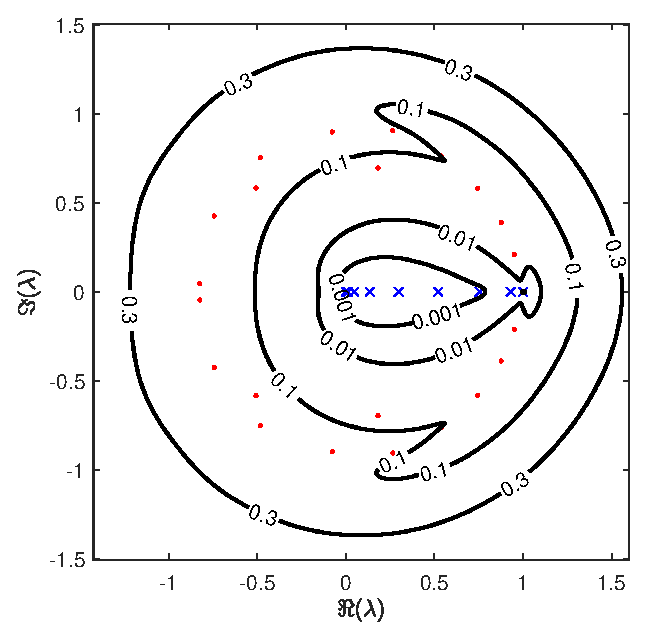
\includegraphics[width=0.55\linewidth]{../code/figures/gauss_map/pseudospectra_contour.eps}
    \end{center}
    \caption{Gauss iterated map problem. Contour lines of the $\varepsilon$-pseudospectrum for $\varepsilon = 0.3,\,0.1,\,0.01,\,0.001$ computed using ResDMD with dictionary of $K=40$ observables.}
\end{figure}
}
\end{frame}

\begin{frame}{Kernelized EDMD (K-EDMD)}
\alert{\textbf{Limitation of EDMD (and ResDMD):}} Need to find a suitable dictionary for each problem.

\medskip
\structure{\textbf{Possible solution:}} Start from a general purpose kernel, such as RBF, and use a two-steps extraction procedure.


\end{frame}
\begin{frame}{Main references}
\nocite{*}
\printbibliography
\end{frame}

\end{document}